\documentclass[10pt,conference]{IEEEtran}

\ifCLASSINFOpdf
  \usepackage[pdftex]{graphicx}
\else
\fi
\usepackage[cmex10]{amsmath}
\usepackage{amsthm,amsfonts,amssymb}
\usepackage{ifthen}
\usepackage{tikz}
\usetikzlibrary{decorations.text}
\usepackage{cite}
\usepackage{amsthm,amsfonts,amssymb}
\setcounter{MaxMatrixCols}{17}
\usepackage{graphicx}
%\usepackage[outdir=./]{epstopdf}
%\usepackage{epigraph}
%\usepackage{tikz}
%\usepackage{natbib}
%\setcitestyle{square}
\usepackage{subfig}
\usepackage{blkarray}
\usepackage{dsfont}
\usepackage[mathscr]{euscript}
\usepackage{enumitem}

\usepackage[top=1in, bottom=1in, left=1in, right=1in]{geometry}
\usepackage{amsfonts}
\usepackage{mathrsfs} 


\usepackage{algorithm}
\usepackage[noend]{algpseudocode}
\usepackage{blkarray}
\usepackage{stfloats}%
%\newtheorem{theorem}{Theorem}
\newtheorem{theorem}{Theorem}[section]
\newtheorem{corollary}{Corollary}[section]
\newtheorem{proposition}{Proposition}[section]
\newtheorem{lemma}{Lemma}[section]
\theoremstyle{remark}
\newtheorem*{remark}{Remark}
\theoremstyle{definition}
\newtheorem{definition}{Definition}[section]
\newtheorem{example}{Example}[section]
\usepackage{url}
\usepackage{tcolorbox}
\usepackage{arydshln}
\usepackage{mathtools}
\usepackage{dsfont}
\definecolor{brickred}{cmyk}{0,0.89,0.94,0.28}
\definecolor{goldenrod}{cmyk}{0,0.10,0.84,0}
\definecolor{purple}{cmyk}{0.45,0.86,0,0}
\definecolor{rawsienna}{cmyk}{0,0.72,1,0.45}
\definecolor{olivegreen}{cmyk}{0.64,0,0.95,0.40}
\definecolor{peach}{cmyk}{0,0.5,0.7,0}
\definecolor{darkolive}{rgb}{0.,0.4,0.}
\colorlet{grey}{gray!40}

\def\tcw{\textcolor{white}}
\def\tcbr{\textcolor{brickred}}
\def\tcbl{\textcolor{blue}}
\def\tcrs{\textcolor{rawsienna}}
\def\tcog{\textcolor{olivegreen}}
\def\tcpl{\textcolor{purple}}
\def\tcgr{\textcolor{grey}}

\DeclareMathOperator{\argmin}{\text{argmin}}

\global\long\def\P{\mathbb{P}}
\global\long\def\E{\mathbb{E}}
\global\long\def\V{\mathrm{Var}}
\global\long\def\C{\mathrm{Cov}}
\global\long\def\I{\mathbbm{1}}
\global\long\def\d{\mathrm{d}}

\usepackage{xcolor}
\newcommand\arv[1]{{\color{red}\textbf{Arvind: #1}}}

\usepackage{xcolor}
\newcommand\pra[1]{{\color{blue}\textbf{Prajjwal: #1}}}

\DeclarePairedDelimiter\ceil{\lceil}{\rceil}
\DeclarePairedDelimiter\floor{\lfloor}{\rfloor} % Use the [cmex10] option to ensure 
\interdisplaylinepenalty=2500

\usepackage[cmintegrals]{newtxmath}



\hyphenation{op-tical net-works semi-conduc-tor}


\begin{document}
\title{Bounding User Contributions for User-Level Differentially Private Mean Estimation}
%\author{
%\IEEEauthorblockN{V.~Arvind~Rameshwar}
%\IEEEauthorblockA{IUDX Program Unit\\IISc, Bengaluru, India\\
%	Email: arvind.rameshwar@gmail.com}
%\and
%\IEEEauthorblockN{Anshoo~Tandon}
%\IEEEauthorblockA{IUDX Program Unit\\IISc, Bengaluru, India\\
%	Email: anshoo.tandon@gmail.com}
%\and
%\IEEEauthorblockN{Abhay~Sharma}
%\IEEEauthorblockA{IUDX Program Unit\\IISc, Bengaluru, India\\
%	Email: abhay.sharma@datakaveri.org}
%}
\author{\IEEEauthorblockN{
		V.~Arvind~Rameshwar\ \
		and\ \ 
		Anshoo~Tandon
	}
	\thanks{The authors are with the India Urban Data Exchange Program Unit, Indian Institute of Science, Bengaluru, India, emails: \texttt{\{arvind.rameshwar, anshoo.tandon\}@gmail.com}.}
}
\IEEEoverridecommandlockouts
\maketitle


\begin{abstract}

We revisit the problem of releasing the sample mean of bounded samples in a dataset, privately, under user-level $\varepsilon$-differential privacy (DP). We aim to derive the optimal method of preprocessing data samples, within a canonical class of processing strategies, in terms of the error in estimation. Typical error analyses of such \emph{bounding} (or \emph{clipping}) strategies in the literature assume that the data samples are independent and identically distributed (i.i.d.), and sometimes also that all users contribute the same number of samples (data homogeneity)---assumptions that do not accurately model real-world data distributions. Our main result in this work is a precise characterization of the preprocessing strategy that gives rise to the smallest \emph{worst-case} error over all datasets -- a \emph{distribution-independent} error metric -- while allowing for data heterogeneity. We also show via experimental studies that even for i.i.d. real-valued samples, our clipping strategy performs much better, in terms of \emph{average-case} error, than the widely used bounding strategy of Amin et al. (2019).
\end{abstract}

% no keywords




% For peer review papers, you can put extra information on the cover
% page as needed:
% \ifCLASSOPTIONpeerreview
% \begin{center} \bfseries EDICS Category: 3-BBND \end{center}
% \fi
%
% For peerreview papers, this IEEEtran command inserts a page break and
% creates the second title. It will be ignored for other modes.
\IEEEpeerreviewmaketitle



\section{Introduction}
%Federated learning (FL) is now a widely studied framework for the collaborative training of a machine learning (ML) model by a large collection of devices (also called clients or users), by using decentralized training data. Typically, such a training task proceeds iteratively; in every round, each participating client performs a local update to the machine learning model using its training data and then sends this update to a central server, which is tasked with ``aggregating" the received updates. The aggregated model is then communicated back to the clients, which then begin a fresh round of local model updates. A canonical FL algorithm is the \texttt{FedAvg} algorithm introduced in \cite{fl-mcmahan}. Importantly, FL allows for the training of a large-scale ML model in a distributed fashion, while ensuring that the training data remains private to each client. For a thorough survey of the challenges in real-world deployment of FL, we refer the reader to \cite{kairouz-survey,li-survey}.

In this article, we concern ourselves with the fundamental problem of processing bounded, potentially vector-valued samples in a dataset, for the release of a private estimate of the sample mean. In particular, we work within the framework of ``user-level" differential privacy \cite{userlevel,hetero}, which is a generalization of the now widely adopted framework of differential privacy (DP) \cite{dworkroth, vadhan2017} for the design and analysis of privacy-preserving algorithms. Loosely speaking, user-level DP guarantees the privacy of a ``user", who could contribute more than one sample, by ensuring the statistical indistinguishability of outputs of the algorithm to changes in the user's samples. User-level DP has practical relevance for inference tasks on most real-world datasets, such as traffic datasets, datasets of user expenditures, and time series data, where different users contribute potentially different numbers of samples (data heterogeneity) \cite{usereg3,usereg4}. Moreover, user-level DP algorithms are increasingly becoming popular subroutines for integration into
federated learning (FL) frameworks -- see, e.g., \cite[Sec. 4]{kairouz-survey} for more details. 

%User-level privacy assumes significance in the context of real-world IoT datasets, such as traffic databases, which record multiple contributions from every user (see also \cite{usereg1,usereg2,usereg3,usereg4}). Specifically, user-level DP mechanisms for mean estimation \cite{userlevel,usereg4} are employed by the central server in a canonical FL algorithm such as \texttt{FedAvg} \cite{fl-mcmahan}, while computing a weighted average of gradients passed by each client; these mechanisms help ensure the privacy of a single user (or client), who potentially contributes several samples to the training dataset. 

There are two key requirements of such user-level DP mechanisms for mean estimation, for real-world applications. Firstly, the mechanisms must be designed to work with heterogeneous data. Secondly, one would like reliable reconstruction of the true sample mean, even when the data samples are non-i.i.d. (independent and identically distributed). Our focus is hence to  characterize an error metric, which is independent of the underlying data distribution and can be explicitly computed and optimized, for heterogeneous data.

%The second requirement is of particular importance in FL applications, where each client would like to reliably reconstruct the aggregated model update, in every round, from the noisy, privatized aggregate released by the central server, while running the FL algorithm on highly correlated real-world datasets.  

In this article, we confine our attention to (pure) $\varepsilon$-DP algorithms for mean estimation. A key subroutine in most user-level $\varepsilon$-DP mechanisms \cite{userlevel,hetero-user-level,hist-user-level,amin} is the preprocessing of the data samples for the release of an estimate of the sample mean, which requires the addition of less noise for privacy (measured via the sensitivity of the estimate), as against releasing a noised version of the true sample mean. Such a preprocessing procedure (also called a strategy for ``bounding" or ``clipping" strategy \cite{amin}) either drops certain samples contributed by selected users, or projects the samples to a ``high-probability interval" that is a strict subset of the interval in which the sample values are known to lie. While it is usually easy to establish that the mechanisms designed using the clipped estimators are differentially private, an analysis of their ``utility", or the error in estimation of the true statistic, often relies on distributional assumptions about the dataset. 

In this work, following \cite{dp_spcom,dp_preprint,tit-preprint}, we define and explicitly compute the \emph{worst-case error}, over all datasets, of general preprocessing (or bounding) strategies. The worst-case error metric is natural in settings with arbitrarily correlated data, where each user potentially ascribes his/her error tolerance to the worst dataset that the statistic is computed on. Furthermore, this error metric is clearly distribution independent and is computable under data heterogeneity too. We then explicitly identify the bounding strategy that results in the smallest worst-case error; our approach is hence an extension of those in \cite{amin} to the setting of the worst-case error, while allowing for arbitrary bounding strategies. Interestingly, we also observe from experimental studies that for scalar samples, our clipping strategy also gives rise to much smaller errors \emph{on average} compared to the strategy in \cite{amin}, for selected dataset sizes, when the samples are drawn i.i.d. according to common distributions.

%In recent work \cite{dp_spcom,dp_preprint,tit-preprint}, the authors introduced the notion of the \emph{worst-case error} incurred by a given mechanism, and showed that such an error metric is explicitly computable for selected clipped, $\varepsilon$-DP estimators for private mean and variance release. Importantly, the worst-case error metric is \emph{independent} of the distribution of the samples in the dataset, and is computable even when the data is heterogeneous. 

%In this work, we generalize the results in \cite{dp_spcom,dp_preprint} by considering clipping strategies that can project or drop data samples, potentially arbitrarily. Our analysis allows us to identify the clipping strategy that results in the smallest worst-case error -- such a strategy simply projects each data sample contributed by a user to an interval determined by the \emph{number} of samples he/she contributes. Our result can be seen as an extension of those in \cite{amin} to the setting of the worst-case error, while allowing for arbitrary bounding strategies. Interestingly, we also observe from experimental studies that our clipping strategy, which does not rely on additional, private parameter estimation unlike that in \cite{amin}, also gives rise to much smaller errors on average as compared to the strategy in \cite{amin}, for selected distributions of numbers of user contributions, when the samples are drawn i.i.d. according to common distributions.

%It is now well-understood that the release of even seemingly innocuous functions of a dataset that is not publicly available can result in the reconstruction of the identities of individuals (or users) in the dataset with alarming levels of accuracy (see, e.g.,  \cite{narayanan, sweeney}). To alleviate concerns over such attacks, the framework of differential privacy (DP) was introduced in \cite{dwork06}, which guarantees the privacy of any single sample. Subsequently, several works (see the surveys \cite{dworkroth, vadhan2017} for references) have designed DP mechanisms for the release of statistics such as the mean, variance, and histograms.




\section{Notation and Preliminaries}
\section{Preliminaries}
\label{sec:prelim}
\label{sec:term}
We define the key terminologies used, primarily focusing on the hidden states (or activations) during the forward pass. 

\paragraph{Components in an attention layer.} We denote $\Res$ as the residual stream. We denote $\Val$ as Value (states), $\Qry$ as Query (states), and $\Key$ as Key (states) in one attention head. The \attlogit~represents the value before the softmax operation and can be understood as the inner product between  $\Qry$  and  $\Key$. We use \Attn~to denote the attention weights of applying the SoftMax function to \attlogit, and ``attention map'' to describe the visualization of the heat map of the attention weights. When referring to the \attlogit~from ``$\tokenB$'' to  ``$\tokenA$'', we indicate the inner product  $\langle\Qry(\tokenB), \Key(\tokenA)\rangle$, specifically the entry in the ``$\tokenB$'' row and ``$\tokenA$'' column of the attention map.

\paragraph{Logit lens.} We use the method of ``Logit Lens'' to interpret the hidden states and value states \citep{belrose2023eliciting}. We use \logit~to denote pre-SoftMax values of the next-token prediction for LLMs. Denote \readout~as the linear operator after the last layer of transformers that maps the hidden states to the \logit. 
The logit lens is defined as applying the readout matrix to residual or value states in middle layers. Through the logit lens, the transformed hidden states can be interpreted as their direct effect on the logits for next-token prediction. 

\paragraph{Terminologies in two-hop reasoning.} We refer to an input like “\Src$\to$\brga, \brgb$\to$\Ed” as a two-hop reasoning chain, or simply a chain. The source entity $\Src$ serves as the starting point or origin of the reasoning. The end entity $\Ed$ represents the endpoint or destination of the reasoning chain. The bridge entity $\Brg$ connects the source and end entities within the reasoning chain. We distinguish between two occurrences of $\Brg$: the bridge in the first premise is called $\brga$, while the bridge in the second premise that connects to $\Ed$ is called $\brgc$. Additionally, for any premise ``$\tokenA \to \tokenB$'', we define $\tokenA$ as the parent node and $\tokenB$ as the child node. Furthermore, if at the end of the sequence, the query token is ``$\tokenA$'', we define the chain ``$\tokenA \to \tokenB$, $\tokenB \to \tokenC$'' as the Target Chain, while all other chains present in the context are referred to as distraction chains. Figure~\ref{fig:data_illustration} provides an illustration of the terminologies.

\paragraph{Input format.}
Motivated by two-hop reasoning in real contexts, we consider input in the format $\bos, \text{context information}, \query, \answer$. A transformer model is trained to predict the correct $\answer$ given the query $\query$ and the context information. The context compromises of $K=5$ disjoint two-hop chains, each appearing once and containing two premises. Within the same chain, the relative order of two premises is fixed so that \Src$\to$\brga~always precedes \brgb$\to$\Ed. The orders of chains are randomly generated, and chains may interleave with each other. The labels for the entities are re-shuffled for every sequence, choosing from a vocabulary size $V=30$. Given the $\bos$ token, $K=5$ two-hop chains, \query, and the \answer~tokens, the total context length is $N=23$. Figure~\ref{fig:data_illustration} also illustrates the data format. 

\paragraph{Model structure and training.} We pre-train a three-layer transformer with a single head per layer. Unless otherwise specified, the model is trained using Adam for $10,000$ steps, achieving near-optimal prediction accuracy. Details are relegated to Appendix~\ref{app:sec_add_training_detail}.


% \RZ{Do we use source entity, target entity, and mediator entity? Or do we use original token, bridge token, end token?}





% \paragraph{Basic notations.} We use ... We use $\ve_i$ to denote one-hot vectors of which only the $i$-th entry equals one, and all other entries are zero. The dimension of $\ve_i$ are usually omitted and can be inferred from contexts. We use $\indicator\{\cdot\}$ to denote the indicator function.

% Let $V > 0$ be a fixed positive integer, and let $\vocab = [V] \defeq \{1, 2, \ldots, V\}$ be the vocabulary. A token $v \in \vocab$ is an integer in $[V]$ and the input studied in this paper is a sequence of tokens $s_{1:T} \defeq (s_1, s_2, \ldots, s_T) \in \vocab^T$ of length $T$. For any set $\mathcal{S}$, we use $\Delta(\mathcal{S})$ to denote the set of distributions over $\mathcal{S}$.

% % to a sequence of vectors $z_1, z_2, \ldots, z_T \in \real^{\dout}$ of dimension $\dout$ and length $T$.

% Let $\mU = [\vu_1, \vu_2, \ldots, \vu_V]^\transpose \in \real^{V\times d}$ denote the token embedding matrix, where the $i$-th row $\vu_i \in \real^d$ represents the $d$-dimensional embedding of token $i \in [V]$. Similarly, let $\mP = [\vp_1, \vp_2, \ldots, \vp_T]^\transpose \in \real^{T\times d}$ denote the positional embedding matrix, where the $i$-th row $\vp_i \in \real^d$ represents the $d$-dimensional embedding of position $i \in [T]$. Both $\mU$ and $\mP$ can be fixed or learnable.

% After receiving an input sequence of tokens $s_{1:T}$, a transformer will first process it using embedding matrices $\mU$ and $\mP$ to obtain a sequence of vectors $\mH = [\vh_1, \vh_2, \ldots, \vh_T] \in \real^{d\times T}$, where 
% \[
% \vh_i = \mU^\transpose\ve_{s_i} + \mP^\transpose\ve_{i} = \vu_{s_i} + \vp_i.
% \]

% We make the following definitions of basic operations in a transformer.

% \begin{definition}[Basic operations in transformers] 
% \label{defn:operators}
% Define the softmax function $\softmax(\cdot): \real^d \to \real^d$ over a vector $\vv \in \real^d$ as
% \[\softmax(\vv)_i = \frac{\exp(\vv_i)}{\sum_{j=1}^d \exp(\vv_j)} \]
% and define the softmax function $\softmax(\cdot): \real^{m\times n} \to \real^{m \times n}$ over a matrix $\mV \in \real^{m\times n}$ as a column-wise softmax operator. For a squared matrix $\mM \in \real^{m\times m}$, the causal mask operator $\mask(\cdot): \real^{m\times m} \to \real^{m\times m}$  is defined as $\mask(\mM)_{ij} = \mM_{ij}$ if $i \leq j$ and  $\mask(\mM)_{ij} = -\infty$ otherwise. For a vector $\vv \in \real^n$ where $n$ is the number of hidden neurons in a layer, we use $\layernorm(\cdot): \real^n \to \real^n$ to denote the layer normalization operator where
% \[
% \layernorm(\vv)_i = \frac{\vv_i-\mu}{\sigma}, \mu = \frac{1}{n}\sum_{j=1}^n \vv_j, \sigma = \sqrt{\frac{1}{n}\sum_{j=1}^n (\vv_j-\mu)^2}
% \]
% and use $\layernorm(\cdot): \real^{n\times m} \to \real^{n\times m}$ to denote the column-wise layer normalization on a matrix.
% We also use $\nonlin(\cdot)$ to denote element-wise nonlinearity such as $\relu(\cdot)$.
% \end{definition}

% The main components of a transformer are causal self-attention heads and MLP layers, which are defined as follows.

% \begin{definition}[Attentions and MLPs]
% \label{defn:attn_mlp} 
% A single-head causal self-attention $\attn(\mH;\mQ,\mK,\mV,\mO)$ parameterized by $\mQ,\mK,\mV \in \real^{{\dqkv\times \din}}$ and $\mO \in \real^{\dout\times\dqkv}$ maps an input matrix $\mH \in \real^{\din\times T}$ to
% \begin{align*}
% &\attn(\mH;\mQ,\mK,\mV,\mO) \\
% =&\mO\mV\layernorm(\mH)\softmax(\mask(\layernorm(\mH)^\transpose\mK^\transpose\mQ\layernorm(\mH))).
% \end{align*}
% Furthermore, a multi-head attention with $M$ heads parameterized by $\{(\mQ_m,\mK_m,\mV_m,\mO_m) \}_{m=1}^M$ is defined as 
% \begin{align*}
%     &\Attn(\mH; \{(\mQ_m,\mK_m,\mV_m,\mO_m) \}_{m\in[M]}) \\ =& \sum_{m=1}^M \attn(\mH;\mQ_m,\mK_m,\mV_m,\mO_m) \in \real^{\dout \times T}.
% \end{align*}
% An MLP layer $\mlp(\mH;\mW_1,\mW_2)$ parameterized by $\mW_1 \in \real^{\dhidden\times \din}$ and $\mW_2 \in \real^{\dout \times \dhidden}$ maps an input matrix $\mH = [\vh_1, \ldots, \vh_T] \in \real^{\din \times T}$ to
% \begin{align*}
%     &\mlp(\mH;\mW_1,\mW_2) = [\vy_1, \ldots, \vy_T], \\ \text{where } &\vy_i = \mW_2\nonlin(\mW_1\layernorm(\vh_i)), \forall i \in [T].
% \end{align*}

% \end{definition}

% In this paper, we assume $\din=\dout=d$ for all attention heads and MLPs to facilitate residual stream unless otherwise specified. Given \Cref{defn:operators,defn:attn_mlp}, we are now able to define a multi-layer transformer.

% \begin{definition}[Multi-layer transformers]
% \label{defn:transformer}
%     An $L$-layer transformer $\transformer(\cdot): \vocab^T \to \Delta(\vocab)$ parameterized by $\mP$, $\mU$, $\{(\mQ_m^{(l)},\mK_m^{(l)},\mV_m^{(l)},\mO_m^{(l)})\}_{m\in[M],l\in[L]}$,  $\{(\mW_1^{(l)},\mW_2^{(l)})\}_{l\in[L]}$ and $\Wreadout \in \real^{V \times d}$ receives a sequence of tokens $s_{1:T}$ as input and predict the next token by outputting a distribution over the vocabulary. The input is first mapped to embeddings $\mH = [\vh_1, \vh_2, \ldots, \vh_T] \in \real^{d\times T}$ by embedding matrices $\mP, \mU$ where 
%     \[
%     \vh_i = \mU^\transpose\ve_{s_i} + \mP^\transpose\ve_{i}, \forall i \in [T].
%     \]
%     For each layer $l \in [L]$, the output of layer $l$, $\mH^{(l)} \in \real^{d\times T}$, is obtained by 
%     \begin{align*}
%         &\mH^{(l)} =  \mH^{(l-1/2)} + \mlp(\mH^{(l-1/2)};\mW_1^{(l)},\mW_2^{(l)}), \\
%         & \mH^{(l-1/2)} = \mH^{(l-1)} + \\ & \quad \Attn(\mH^{(l-1)}; \{(\mQ_m^{(l)},\mK_m^{(l)},\mV_m^{(l)},\mO_m^{(l)}) \}_{m\in[M]}), 
%     \end{align*}
%     where the input $\mH^{(l-1)}$ is the output of the previous layer $l-1$ for $l > 1$ and the input of the first layer $\mH^{(0)} = \mH$. Finally, the output of the transformer is obtained by 
%     \begin{align*}
%         \transformer(s_{1:T}) = \softmax(\Wreadout\vh_T^{(L)})
%     \end{align*}
%     which is a $V$-dimensional vector after softmax representing a distribution over $\vocab$, and $\vh_T^{(L)}$ is the $T$-th column of the output of the last layer, $\mH^{(L)}$.
% \end{definition}



% For each token $v \in \vocab$, there is a corresponding $d_t$-dimensional token embedding vector $\embed(v) \in \mathbb{R}^{d_t}$. Assume the maximum length of the sequence studied in this paper does not exceed $T$. For each position $t \in [T]$, there is a corresponding positional embedding  







\section{Worst-Case Errors of Bounding Strategies}
\label{sec:bound}
%In this section, we present an explicit characterization of the worst-case errors for a broad class of strategies that work by ``bounding" or ``clipping" the contributions of users, as mentioned in the Introduction. In other words, the estimator $\overline{f}$ of $f$ in \eqref{eq:Mbar} is a suitably clipped or bounded version of the sample mean $f$. We then identify that clipping strategy that leads to the smallest worst-case error.
\subsection{On Clipping Strategies}
We work with estimators $\overline{f} = \overline{f}_{\left\{a_j^{(\ell)},b_j^{(\ell)}\right\}}$ of $f$ obtained by bounding user contributions as follows: for each $\ell\in [L]$ and $j\in [m_\ell]$, we let $\overline{\mathbf{x}}_j^{(\ell)}:= {\mathsf{A}_{a_j^{(\ell)},b_j^{(\ell)}}}\left(\mathbf{x}_j^{(\ell)}\right)$, for reals $0\leq a_j^{(\ell)}\leq b_j^{(\ell)}\leq U$. In words, $\overline{\mathbf{x}}_j^{(\ell)}$ is a projection of $\mathbf{x}_j^{(\ell)}$ onto the set $\mathsf{A}_{a_j^{(\ell)},b_j^{(\ell)}}$, which, intuitively, reduces the range of values that $\mathbf{x}_j^{(\ell)}$ can take, and hence its sensitivity too. Figure \ref{fig:proj} shows a pictorial depiction of the annulus $\mathsf{A}_{a_j^{(\ell)},b_j^{(\ell)}}$ when $d=2$ and examples of projections onto the annulus. We then set 
$
\overline{f} = \overline{f}(\mathcal{D}):= \frac{1}{\sum_{\ell'=1}^L m_{\ell'}}\cdot \sum_{\ell=1}^L \sum_{j=1}^{m_\ell} \mathbf{\overline{x}}_j^{(\ell)}.
$
\begin{figure}
	\centering
	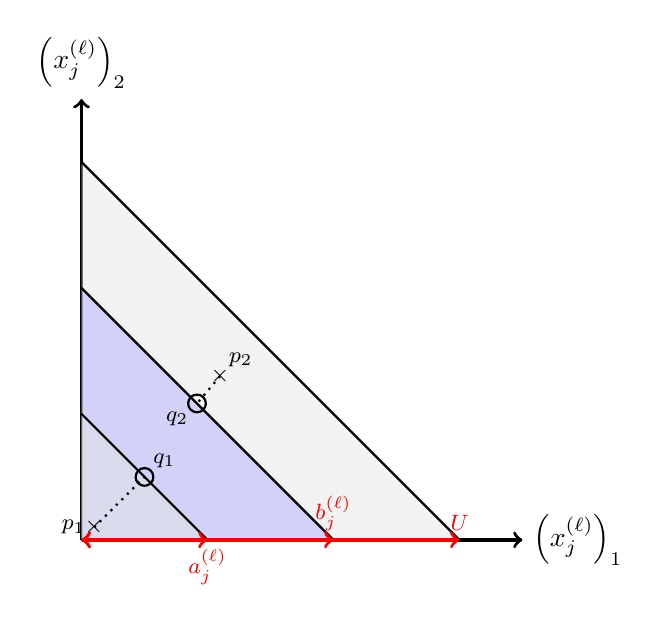
\begin{tikzpicture} [scale=1.6]% Adjust scale as needed
		
		\newcommand{\outerradius}{3}
		\newcommand{\middleradius}{2}
		\newcommand{\innerradius}{1}
		
		% Draw the axes with new labels (only positive quadrant)
		\draw[->, very thick] (0,0) -- (\outerradius+0.5,0) node[right] {$\left(x_j^{(\ell)}\right)_1$};
		\draw[->, very thick] (0,0) -- (0,\outerradius+0.5) node[above] {$\left(x_j^{(\ell)}\right)_2$};
		
		% Draw the balls with transparency (only positive quadrant)
		\draw[thick, fill=gray!20, fill opacity=0.5] (0,\outerradius) -- (\outerradius,0) -- (0,0);
		
		% Draw the blue region *first* (only positive quadrant)
		\fill[blue!30, fill opacity=0.5] (0,\middleradius) -- (\middleradius,0) -- (0,0);
		
		% Draw the inner ball - make it transparent gray (only positive quadrant)
		\draw[thick, fill=gray!20, fill opacity=0.5] (0,\innerradius) -- (\innerradius,0) -- (0,0); % Inner ball
		
		% Draw the middle ball outline in BLACK (only positive quadrant)
		\draw[thick,black] (0,\middleradius) -- (\middleradius,0) -- (0,0);
		
		\footnotesize
		% Add arrows and labels (red, bold tips)
		\draw[<->, very thick, red, line cap=round] (0,0) -- (\innerradius,0) node [below,font=\footnotesize] {$a_j^{(\ell)}$};
		\draw[<->, very thick, red, line cap=round] (0,0) -- (\middleradius,0) node [above,font=\footnotesize] {$b_j^{(\ell)}$};
		
		\draw[<->,very thick, red, line cap=triangle] (0,0) -- (\outerradius,0) node [above,font=\footnotesize] {$U$};
		
		% Mark the point (0.1, 0.1) and line segment
		\draw[thick, black] (0.1,0.1) node {\textbf{$\times$}} node[left] {$p_1$};
		\draw[dotted, thick] (0.1,0.1) -- (0.5,0.5);
		
		% Calculate the endpoint of the second line segment
		\pgfmathsetmacro{\endx}{1.1/1.2}
		\pgfmathsetmacro{\endy}{1.3/1.2}
		
		% Mark the point (1.1, 1.3)/1.2 with a circle
		\draw[thick, black] (\endx,\endy) circle (2pt) node[below left]{$q_2$};
		
		% Mark the point (1.1, 1.3)
		\draw[thick, black] (1.1,1.3) node {\textbf{$\times$}} node[above right]{$p_2$};
		
		% Draw the dotted line segment from (1.1, 1.3)
		\draw[dotted, thick] (1.1,1.3) -- (\endx,\endy);
		
		% Mark the point (0.5, 0.5) with a circle
		\draw[thick, black] (0.5, 0.5) circle (2pt) node[above right]{$q_1$};
		
	\end{tikzpicture}
	\caption{The annulus $\mathsf{A}_{a_j^{(\ell)},b_j^{(\ell)}}$, for $d=2$, shown in blue. Here, the points $q_1$, $q_2$ equal $\mathsf{A}_{a_j^{(\ell)},b_j^{(\ell)}}(p_1)$ and $\mathsf{A}_{a_j^{(\ell)},b_j^{(\ell)}}(p_2)$, respectively.}
	\label{fig:proj}
\end{figure}
Note that the class $\mathsf{B}$ of estimators $\overline{f}$ as above  captures those estimators obtained by dropping selected samples $\mathbf{x}_j^{(\ell)}$ (by setting $a_j^{(\ell)}= b_j^{(\ell)} = 0$ for those samples) and those obtained by projecting samples onto an $\ell_1$-bounded subset of $\Delta_U$, in addition to strategies that perform a combination of dropping and projection. This class of estimators hence includes several common estimators of the sample mean used in works such as \cite{userlevel,dp_preprint,tit-preprint}.

%In the next subsection, we discuss the worst-case errors (as in \eqref{eq:eg}) of mechanisms that employ some $\overline{f}\in \mathsf{B}$ as the estimator of the sample mean.

\subsection{On Worst-Case Errors of Clipping Strategies}
\label{sec:worst-case}
Consider the quantity $E_{\overline{f}}$, for $\overline{f}\in \mathsf{B}$. The following proposition then holds:
\begin{proposition}
	\label{lem:worst-case}
	We have that
	\begin{align*}
		E_{\overline{f}} \notag&= \frac{1}{\sum_{\ell'\leq L} m_{\ell'}}\cdot \left(\sum_{\ell\leq L}\sum_{j\leq m_\ell} \max\left\{a_j^{(\ell)},U-b_j^{(\ell)}\right\}\right)\ + \notag\\
		&\ \ \  \ \ \ \ \ \ \  \ \ \ \ \ \ \ \  \ \ \ \  \ \ \ \frac{d\cdot\max_{\ell\leq L} \sum_{j\leq m_\ell} \left(b_j^{(\ell)}-a_j^{(\ell)}\right)}{\varepsilon\cdot \sum_{\ell'\leq L} m_{\ell'}}.
	\end{align*}
\end{proposition}
The proof of Proposition \ref{lem:worst-case} proceeds with help from a few lemmas. For $E_{\overline{f}}$ as in \eqref{eq:eg}, we define $\beta(\overline{f})$ to be the bias, i.e., $\beta(\overline{f}):= \max_{\mathcal{D}\in \mathsf{D}} \big \lVert f(\mathcal{D}) - \overline{f}(\mathcal{D}) \big\rVert$ and $\eta(\overline{f})$ to be the error due to noise addition, i.e., $\eta(\overline{f}):= \E[\lVert\mathbf{\mathbf{Z}}\rVert_1]$. First, we aim to characterize $\beta(\overline{f})$. To this end, we first state a necessary condition for a vector $\mathbf{y}$ to be an $\ell_1$-projection of a vector $\mathbf{a}\in \Delta_U$ onto $\Delta_\alpha$, for $ \alpha\leq U$. 
\begin{lemma}
	\label{lem:proj1}
	Given $\mathbf{a}\in \Delta_U$ and $\alpha\leq U$, we have $\Delta_\alpha(\mathbf{a}) = \mathbf{a}$, if $\mathbf{a}\in \Delta_{\alpha}$. Else, any $\ell_1$-projection $\mathbf{y} = \Delta_\alpha(\mathbf{a})$ must satisfy $\lVert \mathbf{y}\rVert_1 = \alpha$, with $y_i\leq a_i$, for all $i\in [d]$.
\end{lemma}
\begin{proof}
	The first statement in the lemma is clear. Now, for $\mathbf{a}\notin \Delta_\alpha$, suppose that $\mathbf{y} = \Delta_\alpha(\mathbf{a})$ is such that $\lVert \mathbf{y}\rVert_1 < \alpha$. It can then be seen that by setting $\mathbf{y}':= \lambda\mathbf{y}+(1-\lambda)\mathbf{a}$, for some $\lambda\in (0,1)$ such that $\lVert \mathbf{y}'\rVert_1 = \alpha$, we will obtain that $\lVert \mathbf{y}'-\mathbf{a}\rVert_1 < \lVert \mathbf{y}-\mathbf{a}\rVert_1$, which is a contradiction. Likewise, suppose that $y_i>a_i$, for some $i\in [d]$. Now, consider any coordinate $j\in [d]$ such that $y_j\leq a_j$ (such a coordinate must exist, since $\lVert \mathbf{y}\rVert_1 = \alpha$); by letting $m:= \min\{|y_i-a_i|,|y_j-a_j|\}$ and setting $y_i \gets y_i-m$ and $y_j \gets y_j+m$, we see that we strictly decrease $\lVert \mathbf{y}-\mathbf{a}\rVert_1$, which is a contradiction.
\end{proof}
In the appendix, we explicitly characterize the vectors $\mathbf{y}\in \Delta_\alpha$ that are the $\ell_1$-projections of $\mathbf{a}\in \Delta_U\setminus \Delta_\alpha$, for $\alpha\leq U$; indeed, we have that the condition stated in Lemma \ref{lem:proj1} is both necessary and sufficient. The next lemma exactly characterizes $\beta(\overline{f})$.
\begin{lemma}
	\label{lem:proj2}
	We have that $\beta(\overline{f}) = \frac{1}{\sum_{\ell'\leq L} m_{\ell'}}\cdot \left(\sum_{\ell\leq L}\sum_{j\leq m_\ell} \max\left\{a_j^{(\ell)},U-b_j^{(\ell)}\right\}\right)$.
\end{lemma}
\begin{proof}
	For a sample $\mathbf{x}_j^{(\ell)}\in \mathsf{A}_{a_j^{(\ell)},b_j^{(\ell)}}$, it is clear that $\mathsf{A}_{a_j^{(\ell)},b_j^{(\ell)}}(\mathbf{x}_j^{(\ell)}) = \mathbf{x}_j^{(\ell)}$. Now, suppose that $\mathbf{x}_j^{(\ell)}\in \Delta_U\setminus \Delta_{b_j^{(\ell)}}$. Following Lemma \ref{lem:proj1}, if $\mathbf{y} = \mathsf{A}_{a_j^{(\ell)},b_j^{(\ell)}}(\mathbf{a})$, we must have $\lVert \mathbf{y} - \mathbf{x}_j^{(\ell)}\rVert_1 = \sum_{i\leq d} ((x_j^{(\ell)})_i - y_i) = \lVert \mathbf{x}_j^{(\ell)}\rVert_1 - b_j^{(\ell)}.$ Hence, the worst-case clipping error for sample $\mathbf{x}_j^{(\ell)}$ is $\max\ \lVert \mathsf{A}_{a_j^{(\ell)},b_j^{(\ell)}}(\mathbf{x}_j^{(\ell)}) - \mathbf{x}_j^{(\ell)}\rVert_1 = U-b_j^{(\ell)}$. By symmetric arguments, one can show that if $\mathbf{x}_j^{(\ell)}\in \Delta_{a_j^{(\ell)}}\setminus \delta_{a_j^{(\ell)}}$, we must have $\max\ \lVert \mathsf{A}_{a_j^{(\ell)},b_j^{(\ell)}}(\mathbf{x}_j^{(\ell)}) - \mathbf{x}_j^{(\ell)}\rVert_1 = a_j^{(\ell)}$. Thus, overall, we obtain that 
	\begin{equation}\max_{\mathbf{x}_j^{(\ell)}\in \Delta_U} \lVert \mathsf{A}_{a_j^{(\ell)},b_j^{(\ell)}}(\mathbf{x}_j^{(\ell)}) - \mathbf{x}_j^{(\ell)}\rVert_1 = \max\left\{a_j^{(\ell)},U-b_j^{(\ell)}\right\}. \label{eq:maxclip}\end{equation} 
	Now, for any dataset $\mathcal{D}$, recall that
	\begin{align}
		&\lVert f(\mathcal{D})-\overline{f}(\mathcal{D})\rVert_1 \notag\\
		%&=\frac{1}{\sum_{\ell'\leq L} m_{\ell'}}\left\lVert \sum_{\ell\leq L}\sum_{j\leq m_\ell} \left(\mathbf{x}_j^{(\ell)} - \overline{\mathbf{x}}_j^{(\ell)}\right)\right \rVert_1 \notag\\
		&=\frac{1}{\sum_{\ell'\leq L} m_{\ell'}}\left\lVert \sum_{\ell\leq L}\sum_{j\leq m_\ell} \left(\mathbf{x}_j^{(\ell)} - \mathsf{A}_{a_j^{(\ell)},b_j^{(\ell)}}(\mathbf{x}_j^{(\ell)}) \right)\right \rVert_1. \label{eq:cliphelp}
	\end{align}
	Putting together \eqref{eq:maxclip} and \eqref{eq:cliphelp} concludes the proof.
%	It is then easy to see that the bias
%	\begin{align}
%		&\max_{\mathcal{D}\in \mathsf{D}} |f(\mathcal{D})-\overline{f}(\mathcal{D})| \notag\\&= \frac{1}{\sum_{\ell'\leq L} m_{\ell'}}\cdot \left(\sum_{\ell\leq L}\sum_{j\leq m_\ell} \max\left\{a_j^{(\ell)},U-b_j^{(\ell)}\right\}\right). \label{eq:bias}
%	\end{align}
\end{proof}
The calculation of $\eta(\overline{f})$ is quite similar to the proof above, and is captured in Lemma \ref{lem:proj3} below.

\begin{lemma}
	\label{lem:proj3}
	We have that $\eta(\overline{f}) = \frac{d\cdot \max_{\ell\leq L} \sum_{j\leq m_\ell} \left(b_j^{(\ell)}-a_j^{(\ell)}\right)}{\varepsilon\cdot \sum_{\ell'\leq L} m_{\ell'}}.$
\end{lemma}
\begin{proof}
Via arguments entirely analogous to that in the proof of Lemma \ref{lem:proj2}, the user-level sensitivity of $\overline{f}$ is
$
	\Delta_{\overline{f}} = \frac{\max_{\ell\leq L} \sum_{j\leq m_\ell} \left(b_j^{(\ell)}-a_j^{(\ell)}\right)}{\sum_{\ell'\leq L} m_{\ell'}},
$
since in the worst-case, all samples of a user $\ell$ are changed each from $(a_j^{(\ell)},0,\ldots,0)$ to $(b_j^{(\ell)},0,\ldots,0)$. Using $\E[\lVert \mathbf{Z}\rVert_1] = d\E[|Z_1|] = d\Delta_{\overline{f}} /\varepsilon$ gives us the required result.
\end{proof}
The proof of Proposition \ref{lem:worst-case} then follows directly by putting together Lemmas \ref{lem:proj2} and \ref{lem:proj3}.
%\begin{remark}
%	Via the proof of Lemma \ref{lem:worst-case}, we observe that for a given distribution $\{m_\ell:\ell\in [L]\}$ of user contributions, the dataset $\mathcal{D}$ that gives rise to the largest (or worst-case) error is that where $x_j^{(\ell)} = U$, for all $\ell\in [L]$, $j\in [m_\ell]$. We shall use this observation in the next section when we numerically evaluate the performance of the clipping strategy in \cite{amin} on this ``worst-case dataset".
%\end{remark}


Given the characterization of the worst-case error $E_{\overline{f}}$ as above, we proceed with identifying an estimator $f^\star \in \mathsf{B}$ (equivalently, a bounding strategy) that minimizes $E_{\overline{f}}$, over all $\overline{f}\in \mathsf{B}$. Let $T_\varepsilon$ denote the $\left \lceil \left(\frac{2d}{\varepsilon}\right)\right \rceil^{\text{th}}$-largest value in the collection $\{Um_1,Um_2,\ldots,Um_L\}$; if $\varepsilon<2d/L$, we set $T_\varepsilon = 0$. Our main result is encapsulated in the following theorem:
\begin{theorem}
	\label{thm:opt}
	We have that $f^\star = \overline{f}_{\left\{a_j^{(\ell)},b_j^{(\ell)}\right\}}$ minimizes $E_{\overline{f}}$, where
	$
	a_j^{(\ell)} = \max\left\{\frac{Um_\ell-T_\varepsilon}{2m_\ell},0\right\}\text{ and } b_j^{(\ell)} = \min\left\{\frac{Um_\ell+T_\varepsilon}{2m_\ell},U\right\},
	$
	for all $\ell\in [L]$ and $j\in [m_\ell]$.
\end{theorem}
Some remarks are in order. First, note that the optimal bounding strategy $f^\star$ clips sample values based only on the number of contributions of each user $\ell\in [L]$. Furthermore, note that the interval of projection is determined by $T_\varepsilon$, which is quite similar in structure to the optimal clipping threshold $T$ in \cite{amin} for item-level DP, which is the (privately estimated) $\left \lceil \left(\frac{2}{\varepsilon}\right)\right \rceil^{\text{th}}$-largest \emph{sample value}.

The proof of Theorem \ref{thm:opt} proceeds with help from the following lemma.
\begin{lemma}
	\label{lem:helper}
	There exists an estimator $\overline{f}_{\left\{a_j^{(\ell)},b_j^{(\ell)}\right\}}$ minimizing $E_{\overline{f}}$, which obeys $a_j^{(\ell)}+b_j^{(\ell)} = U$, for all $\ell\in [L]$ and $j\in [m_\ell]$.
\end{lemma}
\begin{proof}
	Consider any optimal estimator $\overline{f}_{\left\{a_j^{(\ell)},b_j^{(\ell)}\right\}}$, and suppose that $a_j^{(\tilde{\ell})}+b_j^{(\tilde{\ell})}>U$, for some $\tilde{\ell}\in [L]$ and $j\in [m_{\tilde{\ell}}]$. The proof when we suppose that $a_j^{(\tilde{\ell})}+b_j^{(\tilde{\ell})}<U$, for some $\tilde{\ell}\in [L]$ and $j\in [m_{\tilde{\ell}}]$, is similar, and is omitted. Let $\delta =  (a_j^{(\tilde{\ell})}+b_j^{(\tilde{\ell})})-U$. By setting $b_j^{(\tilde{\ell})}\gets b_j^{(\tilde{\ell})}-\delta$, we observe that $\beta(\overline{f})$ remains unchanged, while $\eta(\overline{f})$ either remains unchanged or strictly decreases by $\delta>0$.
\end{proof}
Hence, to obtain the explicit structure of an estimator $\overline{f}$ that minimizes $E_{\overline{f}}$, it suffices to focus estimators $\overline{f}_{\left\{a_j^{(\ell)},b_j^{(\ell)}\right\}}$ with $a_j^{(\ell)}+b_j^{(\ell)} = U$, for all $\ell\in [L]$, $j\in [m_\ell]$. For $\ell\in [L]$, let $S^{(\ell)}:= \sum_{j\leq m_\ell} a_j^{(\ell)}$, for any given estimator $\overline{f}$. Then, there exists an estimator $f^\star$ minimizing $E_{\overline{f}}$ that satisfies
\begin{equation}
	\label{eq:optsimp}
	E_{f^\star} = \frac{1}{\sum_{\ell'\leq L} m_{\ell'}}\cdot \left(\sum_{\ell\leq L} S^{(\ell)}+\frac{d}{\varepsilon}\cdot \max_{\ell\leq L} \left(Um_\ell - 2S^{(\ell)}\right)\right).
\end{equation}
We now prove Theorem \ref{thm:opt}.

\begin{proof}[Proof of Thm. \ref{thm:opt}]
	We begin with the expression in \eqref{eq:optsimp}; note that our task now is simply to identify the optimal parameters $\{S^{(\ell)}:\ \ell\in [L]\}$ of $f^\star$ in \eqref{eq:optsimp}. Once these parameters are derived, we simply set $a_j^{(\ell)}:= S^{(\ell)}/m_\ell = U-b_j^{(\ell)}$ (via Lemma \ref{lem:helper}), for each $\ell\in [L]$ and $j\in [m_\ell]$. In the expression in \eqref{eq:optsimp}, let us set $\tau:= \max_{\ell\leq L} \left(Um_\ell - 2S^{(\ell)}\right)$. We hence need to solve the following constrained optimization problem:
	\begin{align}
		&{\text{minimize}}\quad h(\{S^{(\ell)}\}):= \left(\sum_{\ell\leq L} S^{(\ell)}+\frac{d\tau}{\varepsilon}\right)\notag\\
		&\text{subj. to:}\ \  Um_\ell-2S^{(\ell)}\leq \tau,\ S^{(\ell)}\geq 0,\ \forall\ \ell\in [L],\ \tau\geq 0.\label{eq:opt}
	%	&\ \ \ \  \ \ \ \  \ \ \ \ \ \ S\geq 0. \label{eq:opt}
	\end{align}
The optimization problem in \eqref{eq:opt} is a linear programming problem. By standard arguments via the necessity of the KKT conditions \cite[Sec. 5.5.3]{boyd}, there must exist reals $\lambda_\tau\geq 0$ and $\lambda_\ell,\ \mu_\ell\geq 0$, for each $\ell\in [L]$ (or Lagrange multipliers), such that the function $\mathcal{L}(\{S^{(\ell)}\},\ \lambda_\tau,\{\lambda_\ell,\mu_\ell\}):= \sum_{\ell\leq L} S^{(\ell)}+\frac{d\tau}{\varepsilon}-\lambda_\tau \tau\ + \\
\sum_\ell \lambda_\ell\cdot \left(Um_\ell-2S^{(\ell)}-\tau\right)-\sum_\ell \mu_\ell S^{(\ell)}$
%\begin{align*}
%\mathcal{L}(\{S^{(\ell)}\},\ &\lambda_S,\{\lambda_\ell,\mu_\ell\}):= \sum_{\ell\leq L} S^{(\ell)}+\frac{S}{\varepsilon}-\lambda_S S\ + \\
%&\sum_\ell \lambda_\ell\cdot \left(Um_\ell-2S^{(\ell)}-S\right)-\sum_\ell \mu_\ell S^{(\ell)}
%\end{align*}
obeys the following properties.
\begin{itemize}
	\item \textbf{Stationarity}: We have that $\frac{\partial \mathcal{L}}{\partial \tau} = 0$, or $\lambda_\tau+\sum_\ell \lambda_\ell = \frac{d}{\varepsilon},$
%	\begin{equation}
%		\label{eq:stat1}
%		\lambda_S+\sum_\ell \lambda_\ell = \frac{1}{\varepsilon},
%	\end{equation}
and that $\frac{\partial \mathcal{L}}{\partial S^{(\ell)}} = 0$, for each $\ell\in [L]$, or $\lambda_\ell = \frac{1-\mu_\ell}{2}.$
%\begin{equation}
%	\label{eq:stat2}
%	\lambda_\ell = \frac{1-\mu_\ell}{2}.
%\end{equation}
\item \textbf{Complementary slackness}: We have that $	\lambda_\tau \tau= 0,\ \lambda_\ell\cdot \left(Um_\ell-2S^{(\ell)}-\tau\right) = 0,\ \text{and}\ \mu_\ell S^{(\ell)} = 0,$
%\begin{align}
%	\label{eq:comp}
%	\lambda_SS = 0,\ \lambda_\ell\cdot \left(Um_\ell-2S^{(\ell)}-S\right) = 0,\ \text{and}\ \mu_\ell S^{(\ell)} = 0,
%\end{align}
for all $\ell\in [L]$.
\end{itemize}
We claim that the assignment $\tau^\star = T_\varepsilon$ and $S^{(\ell),\star} = \max\left\{\frac{Um_\ell-T_\varepsilon}{2},0\right\}$ satisfies the conditions above, for an appropriate choice of $\lambda_\tau,\{\lambda_\ell,\mu_\ell\}$ values. Indeed, for $\ell\in [L]$, if $S^{(\ell),\star} = 0$, we set $\lambda_\ell = 0$ and $\mu_\ell = 1$; else, we set $\lambda_\ell = \frac12$ and $\mu_\ell = 0$. 
%An optimal choice of parameters $\{a_j^{(\ell)},b_j^{(\ell)}\}$ of an estimator $f^\star$ thus obeys $a_j^{(\ell)}:= \alpha^{(\ell),\star}/m_\ell = U-b_j^{(\ell)}$, for each $\ell\in [L]$ and $j\in [m_\ell]$.
\end{proof}
Observe that from Theorem \ref{thm:opt} and \eqref{eq:optsimp}, the optimal worst-case error is $E^\text{OPT}(\varepsilon)= \frac{1}{\sum_{\ell'\leq L} m_{\ell'}}\cdot\left(\sum_{\ell\leq L} \max\left\{{Um_\ell-T_\varepsilon},0\right\}+\frac{dT_\varepsilon}{\varepsilon}\right).$ %
%\begin{align}
%&E^\text{OPT}(\varepsilon) \notag\\ &= \frac{1}{\sum_{\ell'\leq L} m_{\ell'}}\cdot\left(\sum_{\ell\leq L} \max\left\{\frac{Um_\ell-T_\varepsilon}{2m_\ell},0\right\}+\frac{1}{\varepsilon}\cdot \min_{\ell\leq L} \{T_\varepsilon,Um_\ell\}\right). \label{eq:erropt}
%\end{align}
Note that $T_\varepsilon$ is non-decreasing with $\varepsilon$. The following lemma then holds.
\begin{lemma}
\label{lem:monotonicity}
$E^\text{OPT}(\varepsilon)$ is decreasing with $\varepsilon>0$.
\end{lemma}
\begin{proof}
	Since $T_\varepsilon = Um^\star$, for all $\varepsilon\geq 2d/L$, it can be seen that $E^\text{OPT}(\varepsilon)$ is indeed non-increasing for $\varepsilon\geq 2d/L$.
	
	Now, consider $0<\varepsilon_1<\varepsilon_2<2d/L$; assume for simplicity that we have $m_1\geq m_2\geq \ldots\geq m_L$. Consider the function $g(\varepsilon,t):= \frac{1}{\sum_{\ell'\leq L} m_{\ell'}}\cdot\left(\sum_{\ell\leq L} \max\left\{{Um_\ell-t},0\right\}+\frac{dt}{\varepsilon}\right).$ Then,
	\begin{align*}
		E^\text{OPT}(\varepsilon_2)&= g\left(\varepsilon_2,Um_{\left \lceil \left(\frac{2d}{\varepsilon_2}\right)\right \rceil}\right)\\
		&\leq g\left(\varepsilon_2,Um_{\left \lceil \left(\frac{2d}{\varepsilon_1}\right)\right \rceil}\right)\\
		&< g\left(\varepsilon_1,Um_{\left \lceil \left(\frac{2d}{\varepsilon_1}\right)\right \rceil}\right) = E^\text{OPT}(\varepsilon_1),
	\end{align*}
where the first inequality holds since $t = Um_{\left \lceil \left(\frac{2d}{\varepsilon_2}\right)\right \rceil}$ minimizes $g(\varepsilon_2,t)$, over admissible values of $t$, and the second inequality holds since $\varepsilon_1<\varepsilon_2$.
\end{proof}
%Hence, we obtain that  $E^\text{OPT}(\varepsilon)$ is monotonically non-increasing as a function of $\varepsilon>0$.

A special case of Theorem \ref{thm:opt} is when $d=1$, with the interpretation that each sample $x_j^{(\ell)}\in [0,U]$. Here, the annulus $\mathsf{A}_{a_j^{(\ell)},b_j^{(\ell)}}$ is simply the interval $[a_j^{(\ell)}, b_j^{(\ell)}]\subseteq [0,U]$. This implies that for the case when the samples $\mathbf{x}_j^{(\ell)}$ are allowed to take values in the cube $[0,U]^d$, as against in the $\ell_1$-ball $\lVert \mathbf{x}_j^{(\ell)}\rVert_1\leq U$, one can perform the bounding procedure, using the \emph{same} interval $[a_j^{(\ell)}, b_j^{(\ell)}]$ identified via Theorem \ref{thm:opt} for the $d=1$ setting, for each dimension, independently.
	
%
%	\begin{figure}
%		\centering
%		\begin{tikzpicture} [scale=0.8]% Adjust scale as needed
%			
%			\newcommand{\outerradius}{3}
%			\newcommand{\middleradius}{2}
%			\newcommand{\innerradius}{1}
%			
%			% Draw the axes with new labels
%			\draw[->] (-\outerradius-1,0) -- (\outerradius+1,0) node[right] {$(x_j^{(\ell)})_1$};
%			\draw[->] (0,-\outerradius-1) -- (0,\outerradius+1) node[above] {$(x_j^{(\ell)})_2$};
%			
%			% Draw the balls with transparency
%			\draw[thick, fill=gray!20, fill opacity=0.5] (0,\outerradius) -- (\outerradius,0) -- (0,-\outerradius) -- (-\outerradius,0) -- cycle;
%			
%			% Draw the blue region *first*
%			\fill[blue!30, fill opacity=0.5] (0,\middleradius) -- (\middleradius,0) -- (0,-\middleradius) -- (-\middleradius,0) -- cycle;
%	%		\fill[white] (0,\innerradius) -- (\innerradius,0) -- (0,-\innerradius) -- (-\innerradius,0) -- cycle; % "Cut out" the inner part
%			
%			% Draw the inner ball - make it transparent gray
%			\draw[thick, fill=gray!20, fill opacity=0.5] (0,\innerradius) -- (\innerradius,0) -- (0,-\innerradius) -- (-\innerradius,0) -- cycle; % Inner ball
%			
%			% Draw the middle ball outline in BLACK
%			\draw[thick,black] (0,\middleradius) -- (\middleradius,0) -- (0,-\middleradius) -- (-\middleradius,0) -- cycle;
%			
%			\footnotesize
%			% Add arrows and labels (red, bold tips)
%			\draw[<->, very thick, red, line cap=round] (0,0) -- (\innerradius,0) node [below,font=\footnotesize] {$a_j^{(\ell)}$};
%			\draw[<->, very thick, red, line cap=round] (0,0) -- (\middleradius,0) node [above,font=\footnotesize] {$b_j^{(\ell)}$};
%			
%			\draw[<->,very thick, red, line cap=triangle] (0,0) -- (\outerradius,0) node [above,font=\footnotesize] {$U$};
%			
%			
%		\end{tikzpicture}
%		\caption{The annulus is shown in blue.}
%	\end{figure}


\section{Numerical Experiments}
\section{Experiments}
\label{sec:experiments}
The experiments are designed to address two key research questions.
First, \textbf{RQ1} evaluates whether the average $L_2$-norm of the counterfactual perturbation vectors ($\overline{||\perturb||}$) decreases as the model overfits the data, thereby providing further empirical validation for our hypothesis.
Second, \textbf{RQ2} evaluates the ability of the proposed counterfactual regularized loss, as defined in (\ref{eq:regularized_loss2}), to mitigate overfitting when compared to existing regularization techniques.

% The experiments are designed to address three key research questions. First, \textbf{RQ1} investigates whether the mean perturbation vector norm decreases as the model overfits the data, aiming to further validate our intuition. Second, \textbf{RQ2} explores whether the mean perturbation vector norm can be effectively leveraged as a regularization term during training, offering insights into its potential role in mitigating overfitting. Finally, \textbf{RQ3} examines whether our counterfactual regularizer enables the model to achieve superior performance compared to existing regularization methods, thus highlighting its practical advantage.

\subsection{Experimental Setup}
\textbf{\textit{Datasets, Models, and Tasks.}}
The experiments are conducted on three datasets: \textit{Water Potability}~\cite{kadiwal2020waterpotability}, \textit{Phomene}~\cite{phomene}, and \textit{CIFAR-10}~\cite{krizhevsky2009learning}. For \textit{Water Potability} and \textit{Phomene}, we randomly select $80\%$ of the samples for the training set, and the remaining $20\%$ for the test set, \textit{CIFAR-10} comes already split. Furthermore, we consider the following models: Logistic Regression, Multi-Layer Perceptron (MLP) with 100 and 30 neurons on each hidden layer, and PreactResNet-18~\cite{he2016cvecvv} as a Convolutional Neural Network (CNN) architecture.
We focus on binary classification tasks and leave the extension to multiclass scenarios for future work. However, for datasets that are inherently multiclass, we transform the problem into a binary classification task by selecting two classes, aligning with our assumption.

\smallskip
\noindent\textbf{\textit{Evaluation Measures.}} To characterize the degree of overfitting, we use the test loss, as it serves as a reliable indicator of the model's generalization capability to unseen data. Additionally, we evaluate the predictive performance of each model using the test accuracy.

\smallskip
\noindent\textbf{\textit{Baselines.}} We compare CF-Reg with the following regularization techniques: L1 (``Lasso''), L2 (``Ridge''), and Dropout.

\smallskip
\noindent\textbf{\textit{Configurations.}}
For each model, we adopt specific configurations as follows.
\begin{itemize}
\item \textit{Logistic Regression:} To induce overfitting in the model, we artificially increase the dimensionality of the data beyond the number of training samples by applying a polynomial feature expansion. This approach ensures that the model has enough capacity to overfit the training data, allowing us to analyze the impact of our counterfactual regularizer. The degree of the polynomial is chosen as the smallest degree that makes the number of features greater than the number of data.
\item \textit{Neural Networks (MLP and CNN):} To take advantage of the closed-form solution for computing the optimal perturbation vector as defined in (\ref{eq:opt-delta}), we use a local linear approximation of the neural network models. Hence, given an instance $\inst_i$, we consider the (optimal) counterfactual not with respect to $\model$ but with respect to:
\begin{equation}
\label{eq:taylor}
    \model^{lin}(\inst) = \model(\inst_i) + \nabla_{\inst}\model(\inst_i)(\inst - \inst_i),
\end{equation}
where $\model^{lin}$ represents the first-order Taylor approximation of $\model$ at $\inst_i$.
Note that this step is unnecessary for Logistic Regression, as it is inherently a linear model.
\end{itemize}

\smallskip
\noindent \textbf{\textit{Implementation Details.}} We run all experiments on a machine equipped with an AMD Ryzen 9 7900 12-Core Processor and an NVIDIA GeForce RTX 4090 GPU. Our implementation is based on the PyTorch Lightning framework. We use stochastic gradient descent as the optimizer with a learning rate of $\eta = 0.001$ and no weight decay. We use a batch size of $128$. The training and test steps are conducted for $6000$ epochs on the \textit{Water Potability} and \textit{Phoneme} datasets, while for the \textit{CIFAR-10} dataset, they are performed for $200$ epochs.
Finally, the contribution $w_i^{\varepsilon}$ of each training point $\inst_i$ is uniformly set as $w_i^{\varepsilon} = 1~\forall i\in \{1,\ldots,m\}$.

The source code implementation for our experiments is available at the following GitHub repository: \url{https://anonymous.4open.science/r/COCE-80B4/README.md} 

\subsection{RQ1: Counterfactual Perturbation vs. Overfitting}
To address \textbf{RQ1}, we analyze the relationship between the test loss and the average $L_2$-norm of the counterfactual perturbation vectors ($\overline{||\perturb||}$) over training epochs.

In particular, Figure~\ref{fig:delta_loss_epochs} depicts the evolution of $\overline{||\perturb||}$ alongside the test loss for an MLP trained \textit{without} regularization on the \textit{Water Potability} dataset. 
\begin{figure}[ht]
    \centering
    \includegraphics[width=0.85\linewidth]{img/delta_loss_epochs.png}
    \caption{The average counterfactual perturbation vector $\overline{||\perturb||}$ (left $y$-axis) and the cross-entropy test loss (right $y$-axis) over training epochs ($x$-axis) for an MLP trained on the \textit{Water Potability} dataset \textit{without} regularization.}
    \label{fig:delta_loss_epochs}
\end{figure}

The plot shows a clear trend as the model starts to overfit the data (evidenced by an increase in test loss). 
Notably, $\overline{||\perturb||}$ begins to decrease, which aligns with the hypothesis that the average distance to the optimal counterfactual example gets smaller as the model's decision boundary becomes increasingly adherent to the training data.

It is worth noting that this trend is heavily influenced by the choice of the counterfactual generator model. In particular, the relationship between $\overline{||\perturb||}$ and the degree of overfitting may become even more pronounced when leveraging more accurate counterfactual generators. However, these models often come at the cost of higher computational complexity, and their exploration is left to future work.

Nonetheless, we expect that $\overline{||\perturb||}$ will eventually stabilize at a plateau, as the average $L_2$-norm of the optimal counterfactual perturbations cannot vanish to zero.

% Additionally, the choice of employing the score-based counterfactual explanation framework to generate counterfactuals was driven to promote computational efficiency.

% Future enhancements to the framework may involve adopting models capable of generating more precise counterfactuals. While such approaches may yield to performance improvements, they are likely to come at the cost of increased computational complexity.


\subsection{RQ2: Counterfactual Regularization Performance}
To answer \textbf{RQ2}, we evaluate the effectiveness of the proposed counterfactual regularization (CF-Reg) by comparing its performance against existing baselines: unregularized training loss (No-Reg), L1 regularization (L1-Reg), L2 regularization (L2-Reg), and Dropout.
Specifically, for each model and dataset combination, Table~\ref{tab:regularization_comparison} presents the mean value and standard deviation of test accuracy achieved by each method across 5 random initialization. 

The table illustrates that our regularization technique consistently delivers better results than existing methods across all evaluated scenarios, except for one case -- i.e., Logistic Regression on the \textit{Phomene} dataset. 
However, this setting exhibits an unusual pattern, as the highest model accuracy is achieved without any regularization. Even in this case, CF-Reg still surpasses other regularization baselines.

From the results above, we derive the following key insights. First, CF-Reg proves to be effective across various model types, ranging from simple linear models (Logistic Regression) to deep architectures like MLPs and CNNs, and across diverse datasets, including both tabular and image data. 
Second, CF-Reg's strong performance on the \textit{Water} dataset with Logistic Regression suggests that its benefits may be more pronounced when applied to simpler models. However, the unexpected outcome on the \textit{Phoneme} dataset calls for further investigation into this phenomenon.


\begin{table*}[h!]
    \centering
    \caption{Mean value and standard deviation of test accuracy across 5 random initializations for different model, dataset, and regularization method. The best results are highlighted in \textbf{bold}.}
    \label{tab:regularization_comparison}
    \begin{tabular}{|c|c|c|c|c|c|c|}
        \hline
        \textbf{Model} & \textbf{Dataset} & \textbf{No-Reg} & \textbf{L1-Reg} & \textbf{L2-Reg} & \textbf{Dropout} & \textbf{CF-Reg (ours)} \\ \hline
        Logistic Regression   & \textit{Water}   & $0.6595 \pm 0.0038$   & $0.6729 \pm 0.0056$   & $0.6756 \pm 0.0046$  & N/A    & $\mathbf{0.6918 \pm 0.0036}$                     \\ \hline
        MLP   & \textit{Water}   & $0.6756 \pm 0.0042$   & $0.6790 \pm 0.0058$   & $0.6790 \pm 0.0023$  & $0.6750 \pm 0.0036$    & $\mathbf{0.6802 \pm 0.0046}$                    \\ \hline
%        MLP   & \textit{Adult}   & $0.8404 \pm 0.0010$   & $\mathbf{0.8495 \pm 0.0007}$   & $0.8489 \pm 0.0014$  & $\mathbf{0.8495 \pm 0.0016}$     & $0.8449 \pm 0.0019$                    \\ \hline
        Logistic Regression   & \textit{Phomene}   & $\mathbf{0.8148 \pm 0.0020}$   & $0.8041 \pm 0.0028$   & $0.7835 \pm 0.0176$  & N/A    & $0.8098 \pm 0.0055$                     \\ \hline
        MLP   & \textit{Phomene}   & $0.8677 \pm 0.0033$   & $0.8374 \pm 0.0080$   & $0.8673 \pm 0.0045$  & $0.8672 \pm 0.0042$     & $\mathbf{0.8718 \pm 0.0040}$                    \\ \hline
        CNN   & \textit{CIFAR-10} & $0.6670 \pm 0.0233$   & $0.6229 \pm 0.0850$   & $0.7348 \pm 0.0365$   & N/A    & $\mathbf{0.7427 \pm 0.0571}$                     \\ \hline
    \end{tabular}
\end{table*}

\begin{table*}[htb!]
    \centering
    \caption{Hyperparameter configurations utilized for the generation of Table \ref{tab:regularization_comparison}. For our regularization the hyperparameters are reported as $\mathbf{\alpha/\beta}$.}
    \label{tab:performance_parameters}
    \begin{tabular}{|c|c|c|c|c|c|c|}
        \hline
        \textbf{Model} & \textbf{Dataset} & \textbf{No-Reg} & \textbf{L1-Reg} & \textbf{L2-Reg} & \textbf{Dropout} & \textbf{CF-Reg (ours)} \\ \hline
        Logistic Regression   & \textit{Water}   & N/A   & $0.0093$   & $0.6927$  & N/A    & $0.3791/1.0355$                     \\ \hline
        MLP   & \textit{Water}   & N/A   & $0.0007$   & $0.0022$  & $0.0002$    & $0.2567/1.9775$                    \\ \hline
        Logistic Regression   &
        \textit{Phomene}   & N/A   & $0.0097$   & $0.7979$  & N/A    & $0.0571/1.8516$                     \\ \hline
        MLP   & \textit{Phomene}   & N/A   & $0.0007$   & $4.24\cdot10^{-5}$  & $0.0015$    & $0.0516/2.2700$                    \\ \hline
       % MLP   & \textit{Adult}   & N/A   & $0.0018$   & $0.0018$  & $0.0601$     & $0.0764/2.2068$                    \\ \hline
        CNN   & \textit{CIFAR-10} & N/A   & $0.0050$   & $0.0864$ & N/A    & $0.3018/
        2.1502$                     \\ \hline
    \end{tabular}
\end{table*}

\begin{table*}[htb!]
    \centering
    \caption{Mean value and standard deviation of training time across 5 different runs. The reported time (in seconds) corresponds to the generation of each entry in Table \ref{tab:regularization_comparison}. Times are }
    \label{tab:times}
    \begin{tabular}{|c|c|c|c|c|c|c|}
        \hline
        \textbf{Model} & \textbf{Dataset} & \textbf{No-Reg} & \textbf{L1-Reg} & \textbf{L2-Reg} & \textbf{Dropout} & \textbf{CF-Reg (ours)} \\ \hline
        Logistic Regression   & \textit{Water}   & $222.98 \pm 1.07$   & $239.94 \pm 2.59$   & $241.60 \pm 1.88$  & N/A    & $251.50 \pm 1.93$                     \\ \hline
        MLP   & \textit{Water}   & $225.71 \pm 3.85$   & $250.13 \pm 4.44$   & $255.78 \pm 2.38$  & $237.83 \pm 3.45$    & $266.48 \pm 3.46$                    \\ \hline
        Logistic Regression   & \textit{Phomene}   & $266.39 \pm 0.82$ & $367.52 \pm 6.85$   & $361.69 \pm 4.04$  & N/A   & $310.48 \pm 0.76$                    \\ \hline
        MLP   &
        \textit{Phomene} & $335.62 \pm 1.77$   & $390.86 \pm 2.11$   & $393.96 \pm 1.95$ & $363.51 \pm 5.07$    & $403.14 \pm 1.92$                     \\ \hline
       % MLP   & \textit{Adult}   & N/A   & $0.0018$   & $0.0018$  & $0.0601$     & $0.0764/2.2068$                    \\ \hline
        CNN   & \textit{CIFAR-10} & $370.09 \pm 0.18$   & $395.71 \pm 0.55$   & $401.38 \pm 0.16$ & N/A    & $1287.8 \pm 0.26$                     \\ \hline
    \end{tabular}
\end{table*}

\subsection{Feasibility of our Method}
A crucial requirement for any regularization technique is that it should impose minimal impact on the overall training process.
In this respect, CF-Reg introduces an overhead that depends on the time required to find the optimal counterfactual example for each training instance. 
As such, the more sophisticated the counterfactual generator model probed during training the higher would be the time required. However, a more advanced counterfactual generator might provide a more effective regularization. We discuss this trade-off in more details in Section~\ref{sec:discussion}.

Table~\ref{tab:times} presents the average training time ($\pm$ standard deviation) for each model and dataset combination listed in Table~\ref{tab:regularization_comparison}.
We can observe that the higher accuracy achieved by CF-Reg using the score-based counterfactual generator comes with only minimal overhead. However, when applied to deep neural networks with many hidden layers, such as \textit{PreactResNet-18}, the forward derivative computation required for the linearization of the network introduces a more noticeable computational cost, explaining the longer training times in the table.

\subsection{Hyperparameter Sensitivity Analysis}
The proposed counterfactual regularization technique relies on two key hyperparameters: $\alpha$ and $\beta$. The former is intrinsic to the loss formulation defined in (\ref{eq:cf-train}), while the latter is closely tied to the choice of the score-based counterfactual explanation method used.

Figure~\ref{fig:test_alpha_beta} illustrates how the test accuracy of an MLP trained on the \textit{Water Potability} dataset changes for different combinations of $\alpha$ and $\beta$.

\begin{figure}[ht]
    \centering
    \includegraphics[width=0.85\linewidth]{img/test_acc_alpha_beta.png}
    \caption{The test accuracy of an MLP trained on the \textit{Water Potability} dataset, evaluated while varying the weight of our counterfactual regularizer ($\alpha$) for different values of $\beta$.}
    \label{fig:test_alpha_beta}
\end{figure}

We observe that, for a fixed $\beta$, increasing the weight of our counterfactual regularizer ($\alpha$) can slightly improve test accuracy until a sudden drop is noticed for $\alpha > 0.1$.
This behavior was expected, as the impact of our penalty, like any regularization term, can be disruptive if not properly controlled.

Moreover, this finding further demonstrates that our regularization method, CF-Reg, is inherently data-driven. Therefore, it requires specific fine-tuning based on the combination of the model and dataset at hand.
\section{Conclusion}
\section{Conclusion}
In this work, we propose a simple yet effective approach, called SMILE, for graph few-shot learning with fewer tasks. Specifically, we introduce a novel dual-level mixup strategy, including within-task and across-task mixup, for enriching the diversity of nodes within each task and the diversity of tasks. Also, we incorporate the degree-based prior information to learn expressive node embeddings. Theoretically, we prove that SMILE effectively enhances the model's generalization performance. Empirically, we conduct extensive experiments on multiple benchmarks and the results suggest that SMILE significantly outperforms other baselines, including both in-domain and cross-domain few-shot settings.


%\section*{Acknowledgment}


%The authors would like to thank...





% trigger a \newpage just before the given reference
% number - used to balance the columns on the last page
% adjust value as needed - may need to be readjusted if
% the document is modified later
%\IEEEtriggeratref{8}
% The "triggered" command can be changed if desired:
%\IEEEtriggercmd{\enlargethispage{-5in}}

% references section

% can use a bibliography generated by BibTeX as a .bbl file
% BibTeX documentation can be easily obtained at:
% http://mirror.ctan.org/biblio/bibtex/contrib/doc/
% The IEEEtran BibTeX style support page is at:
% http://www.michaelshell.org/tex/ieeetran/bibtex/
%\bibliographystyle{IEEEtran}
% argument is your BibTeX string definitions and bibliography dataset(s)
%\bibliography{IEEEabrv,../bib/paper}
%
% <OR> manually copy in the resultant .bbl file
% set second argument of \begin to the number of references
% (used to reserve space for the reference number labels box)
\bibliographystyle{IEEEtran}
{\footnotesize
	\bibliography{references}}
\appendix
\section{Characterizing $\ell_1$-Projections Onto $\Delta_\alpha$}
\label{app:projection}
In this section, we argue that the condition in the second statement of Lemma \ref{lem:proj1} is sufficient for the vector $\mathbf{y}$ to be an $\ell_1$-projection of $\mathbf{a}\in \Delta_U\setminus \Delta_\alpha$, for $\alpha\leq U$.

Following Lemma \ref{lem:proj1}, consider the collection $\mathcal{S}\subseteq \mathbb{R}^d$ of points defined as $\mathcal{S}:= \{\mathbf{z}\in \delta_\alpha:\ z_i\leq a_i,\ \text{for all $i\in [d]$}\}$. Note that  when $a_i>\alpha$, for all $i\in [d]$, we have $\mathcal{S} = \delta_\alpha$. Observe that $\mathcal{S}$ is a convex subset of $\mathbb{R}^d$; hence, by a version of Carath\'eodory's Theorem (see the remark after \cite[Thm. 15.3.5]{cover_thomas} and \cite{carath}), any point $\mathbf{z}$ in $\mathcal{S}$ can be written as a convex combination of finitely many, in particular, $d$ points in $\mathcal{S}$. Hence, consider any such collection $\mathcal{Z} = \{\mathbf{z}_1,\ldots,\mathbf{z}_d\}$ whose convex hull equals $\mathcal{S}$. The following claim then holds.
%Now, consider the case where $\mathbf{a}$ is such that $a_i\leq \alpha$, for some $i\in [d]$, and hence that $a_j\geq \alpha$, for some $j\in [d], j\neq i$.  the proof of the sufficiency of the second statement of Lemma \ref{lem:proj1} for this case is similar to that for the first case, and is omitted.

%For the first case above, consider the collection $\mathcal{Z} = \{\mathbf{z}_1,\ldots,\mathbf{z}_d\}$. Here, for $k\neq i$, we define $\mathbf{z}_k = (z_{k,1},\ldots,z_{k,d})$ to be such that $z_{k,i} = a_i$ and $z_{k,k} = \alpha-a_i$,  with $z_{k,r} = 0$, for $r\notin \{i,k\}$. We define $\mathbf{z}_i = (z_{i,1},\ldots,z_{i,d})$ to obey $z_{i,j} = \alpha$, with $z_{i,r} = 0$, for $r\neq j$. 

\begin{proposition}
	\label{prop:proj1}
	For any $\mathbf{z}\in \mathcal{S}$, we have that $\lVert \mathbf{a} - \mathbf{z}\rVert_1$ is a constant.
\end{proposition}
\begin{proof}
	Recall that by the version of Carath\'eodory's Theorem above, any point $\mathbf{z}\in \mathcal{S}$ can be written as $\mathbf{z} = \sum_{k=1}^d \lambda_k \mathbf{z}_k$, where $\lambda_k\geq 0$, with $\sum_{k\leq d} \lambda_k = 1$.  It suffices to show that $\lVert \mathbf{a} - \mathbf{z}\rVert_1$ is independent of $\{\lambda_k\}$. To see this, note that
	\begin{align*}
		\lVert \mathbf{a} - \mathbf{z}\rVert_1&= \sum_{r\leq d} (a_r-z_r)\\
		&=\sum_{r\leq d} (a_r-\sum_{k\leq d} \lambda_k z_{k,r})\\
		&= \sum_{r\leq d} a_r - \sum_{k\leq d} \lambda_k\cdot \sum_{r\leq d} z_{k,r} = \lVert \mathbf{a}\rVert_1 - \alpha,
	\end{align*}
which is independent of $\{\lambda_k\}$.
\end{proof}
We hence have that the condition in Lemma \ref{lem:proj1} is sufficient for the vector $\mathbf{y}$ in its statement to be an $\ell_1$-projection of $\mathbf{a}$. In practice, given a vector $\mathbf{a}\in \Delta_U\setminus \Delta_\alpha$, one can use the vector $\mathbf{y} = \frac{\alpha}{\lVert \mathbf{a}\rVert_1} \mathbf{a}$ as an $\ell_1$-projection.
%\clearpage
%\appendices
%\section{Proof of convexity of $\Phi$}
%\input{app-convex.tex}
%\section{Improving $\ell_2$-Error Using Multiple Noisy Views}
%\input{honaker.tex}
%\section{Proof of Lemma \ref{lem:intnoncommon}}
%\input{intnoncommon.tex}
% that's all folks
\end{document}


